\documentclass{beamer}
\usepackage{color}
\usepackage{hyperref}
% \usepackage{pgf, pgfarrows, pgfnodes}
\usepackage{mathtools}
\usetheme{AnnArbor}
\title[https://github.com/cheraaqee/popSR]{Perceptually-Optimized Loss Function for Image Super-Resolution}
\author[ICSPIS2021]{\small Amirhossein Arezoomand \inst{1} \and Pooryaa Cheraaqee \inst{1} \and Azadeh Mansouri \inst{1}}
\institute[]{\inst{1} \textbf{Department of\\ Electrical and Computer Engineering,\\ Kharazmi University}}
% \date{\today}
\begin{document}
%%%%
\begin{frame}
\frametitle{ICSPIS 2021}
\titlepage
\end{frame}
%%%%
\section*{Outline}
\begin{frame}
\frametitle{Outline}
\tableofcontents[pausesections]
\end{frame}
%%%
\section{Problem Definition}
\subsection{Image Super-Resolution}
\begin{frame}
\frametitle{What is \emph{Super-Resolution}?}
\begin{itemize}
\visible<1->{
\item increasing the dimension}
\begin{itemize}
\visible<2,3>{
\item $\text{input (}X_{M\times N}) \xrightarrow{\text{upsampling by a factor of 2 (i.e. }2\uparrow)} \text{output (}Y_{2M\times 2N})$}
\visible<3>{
\item BiLinear, BiCubic, etc.}
\end{itemize}
\visible<4->{
\item
\textcolor{red}{\textbf{!! Preserving the quality !!}}}
\end{itemize}
\visible<5->{
\begin{center}
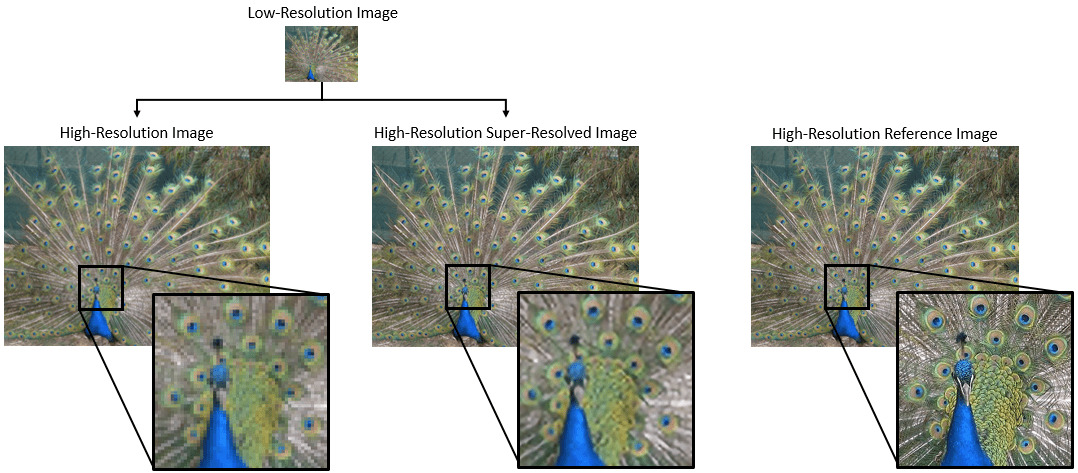
\includegraphics[height=4cm]{sr_sample}
\end{center}
}
\end{frame}
\subsection{Loss Function}
\begin{frame}
\frametitle{CNNs and Loss Functions}
\begin{itemize}
\visible<1->{
\item Super-Resolver CNNs
\vskip 0.5cm
	\only<2-5>{
		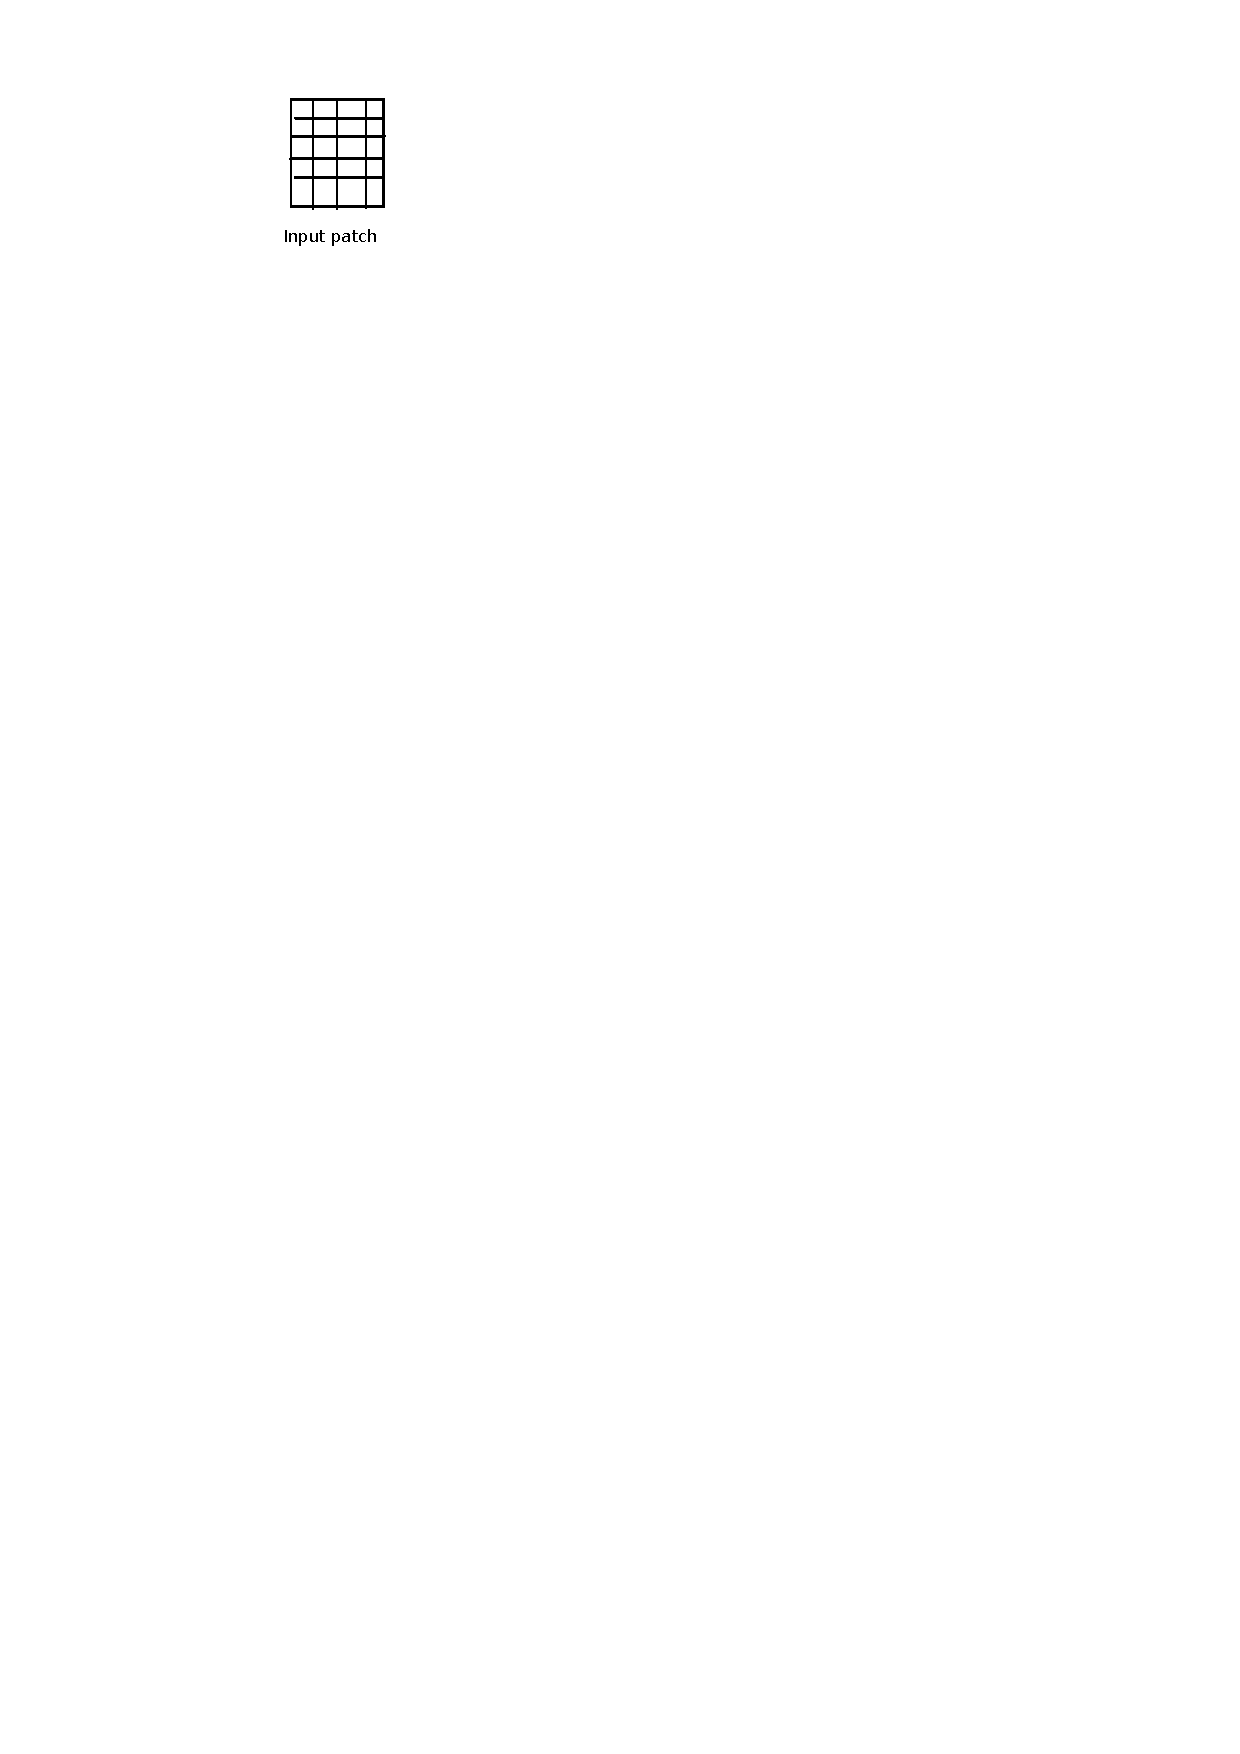
\includegraphics[trim={4.7cm, 25.5cm, 14.5cm, 2cm}, clip, width=1cm]{figure_slide}}
	\only<3-5>{
		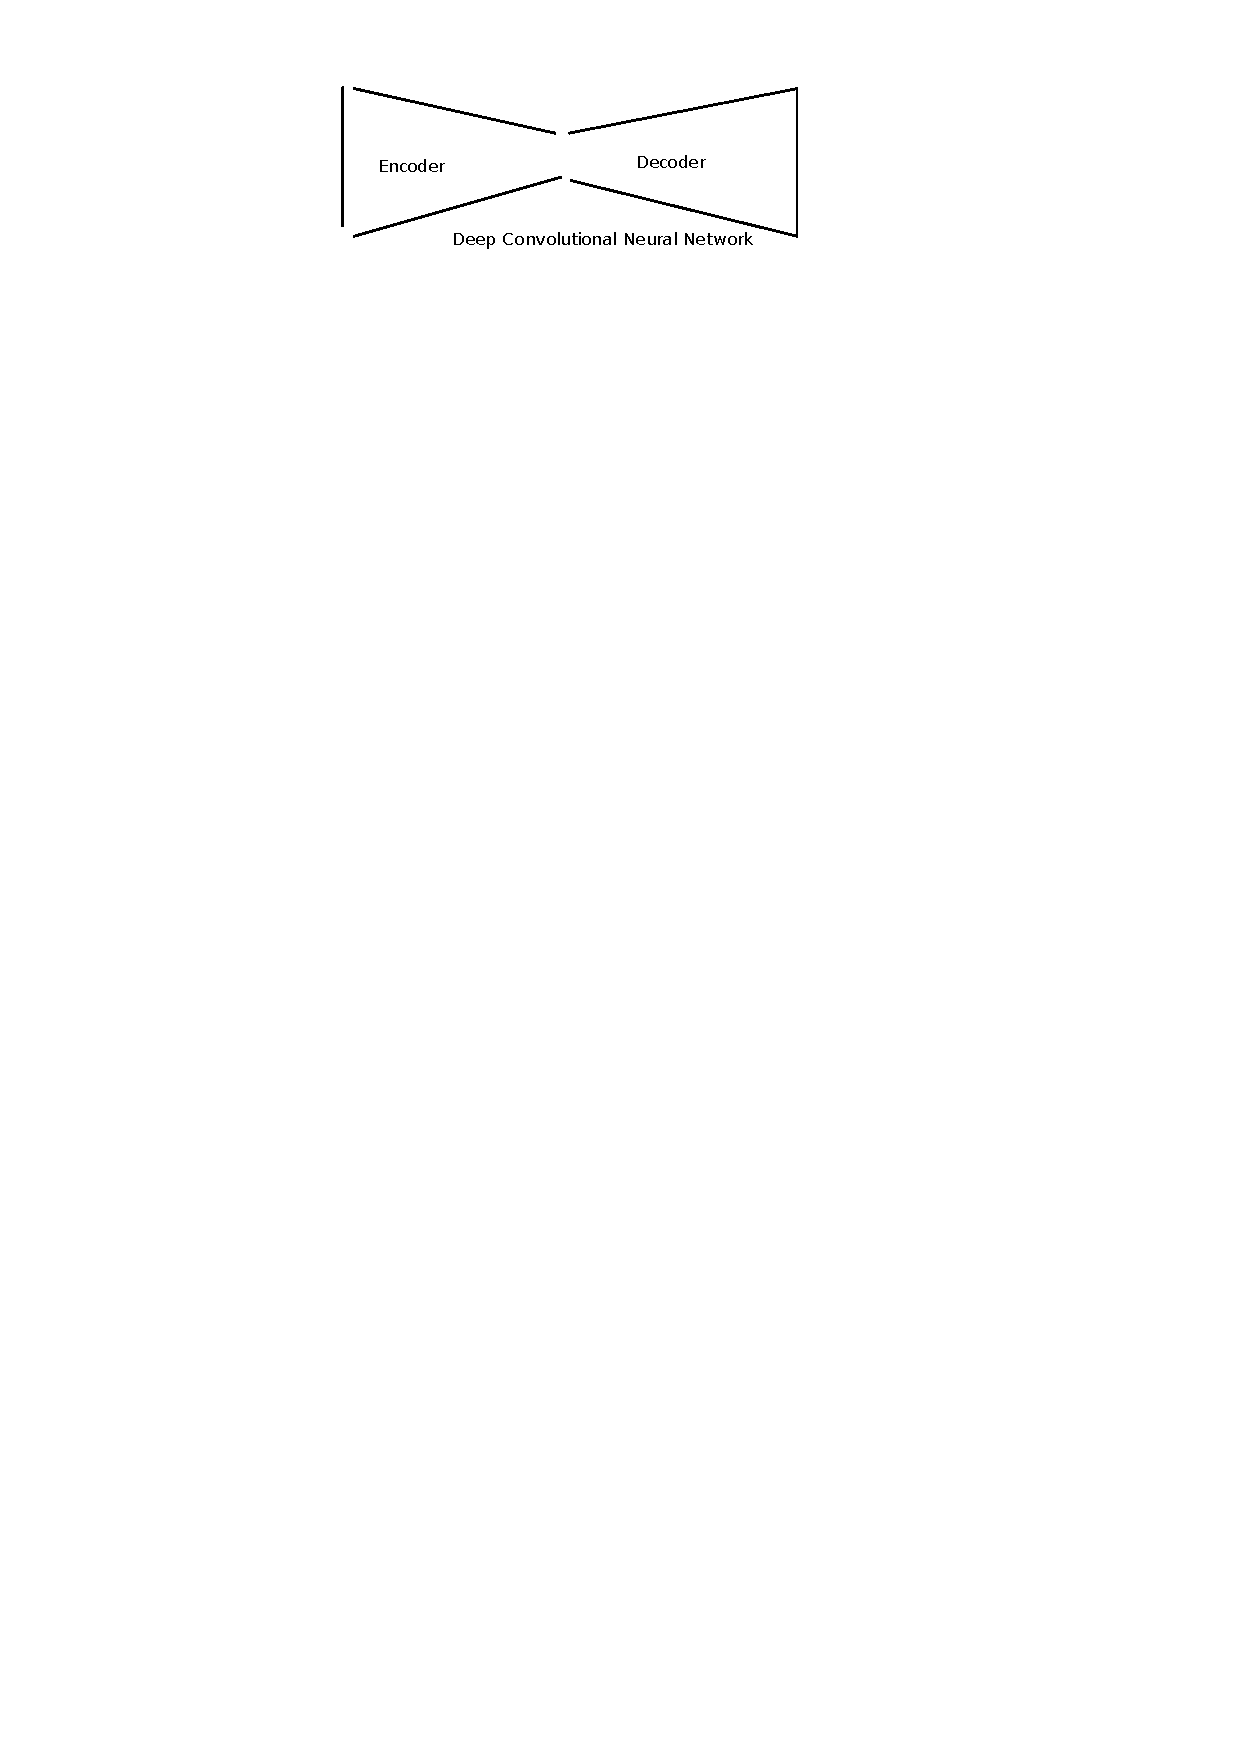
\includegraphics[trim={5.7cm, 25.5cm, 7.3cm, 1.3cm}, clip,width=5cm]{figure_Cnn}}
	\only<4-5>{
		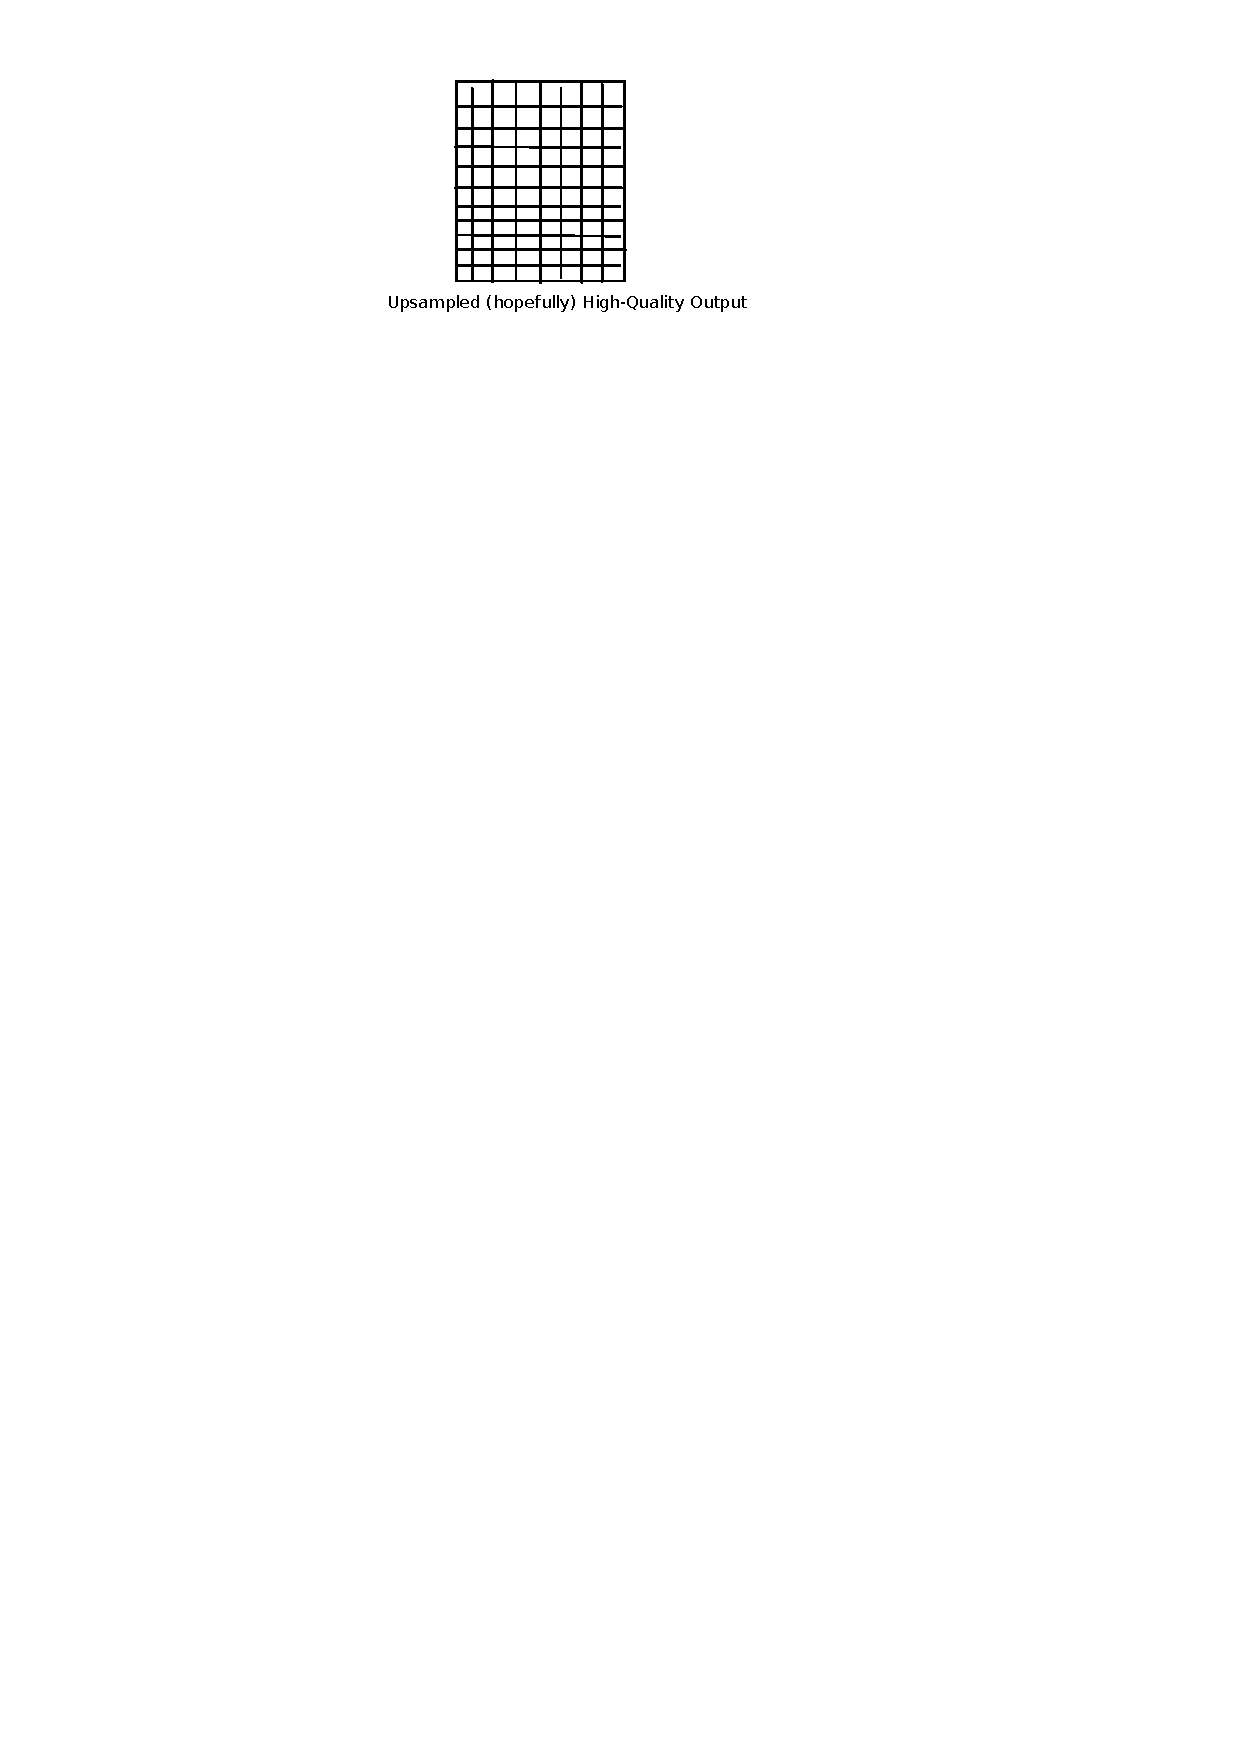
\includegraphics[trim={6.55cm, 24.3cm, 8.2cm, 1.2cm}, clip, width=3cm]{figure_output}}

	\only<5>{
		\hskip 6.5cm 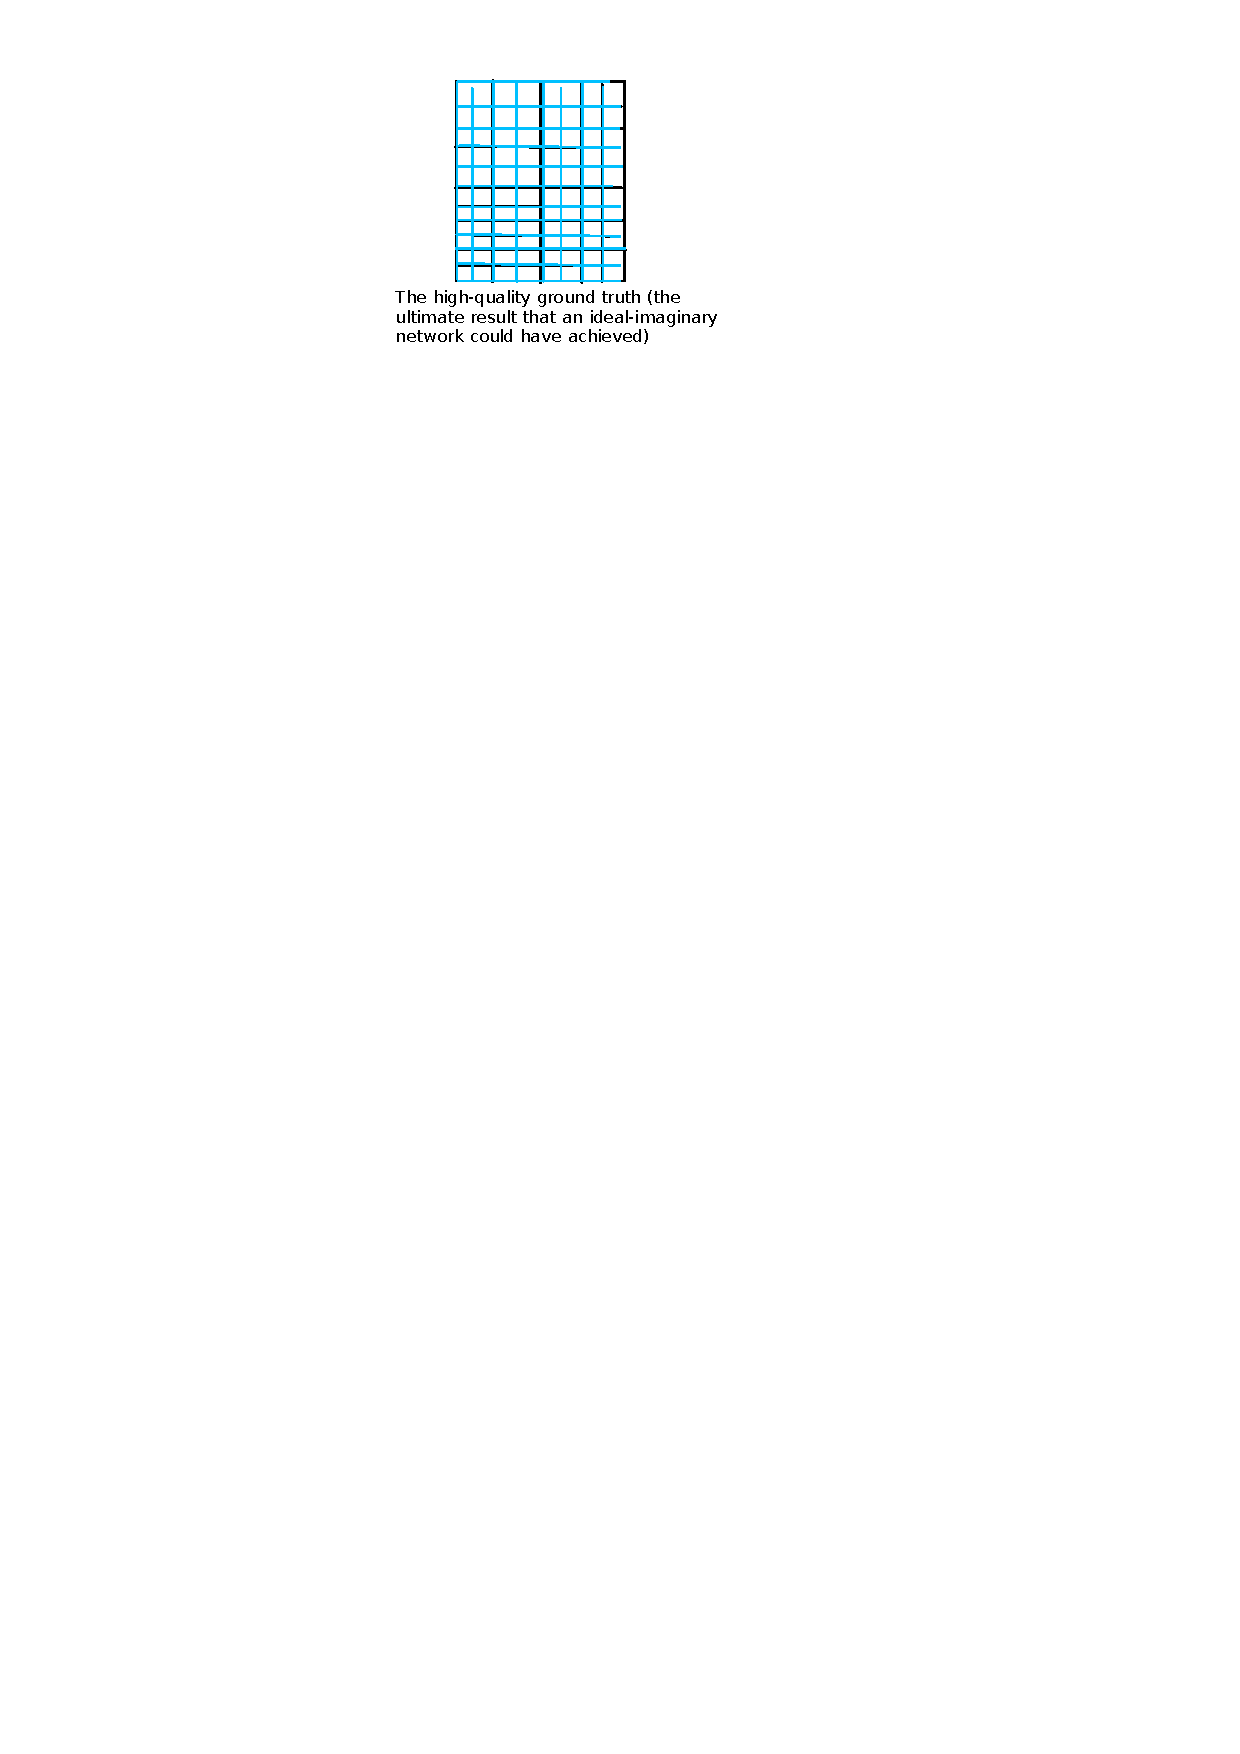
\includegraphics[trim={6.55cm, 23.3cm, 8.5cm, 1.2cm}, clip, width=3cm]{figure_gt}}
}
% \visible<6->{
% 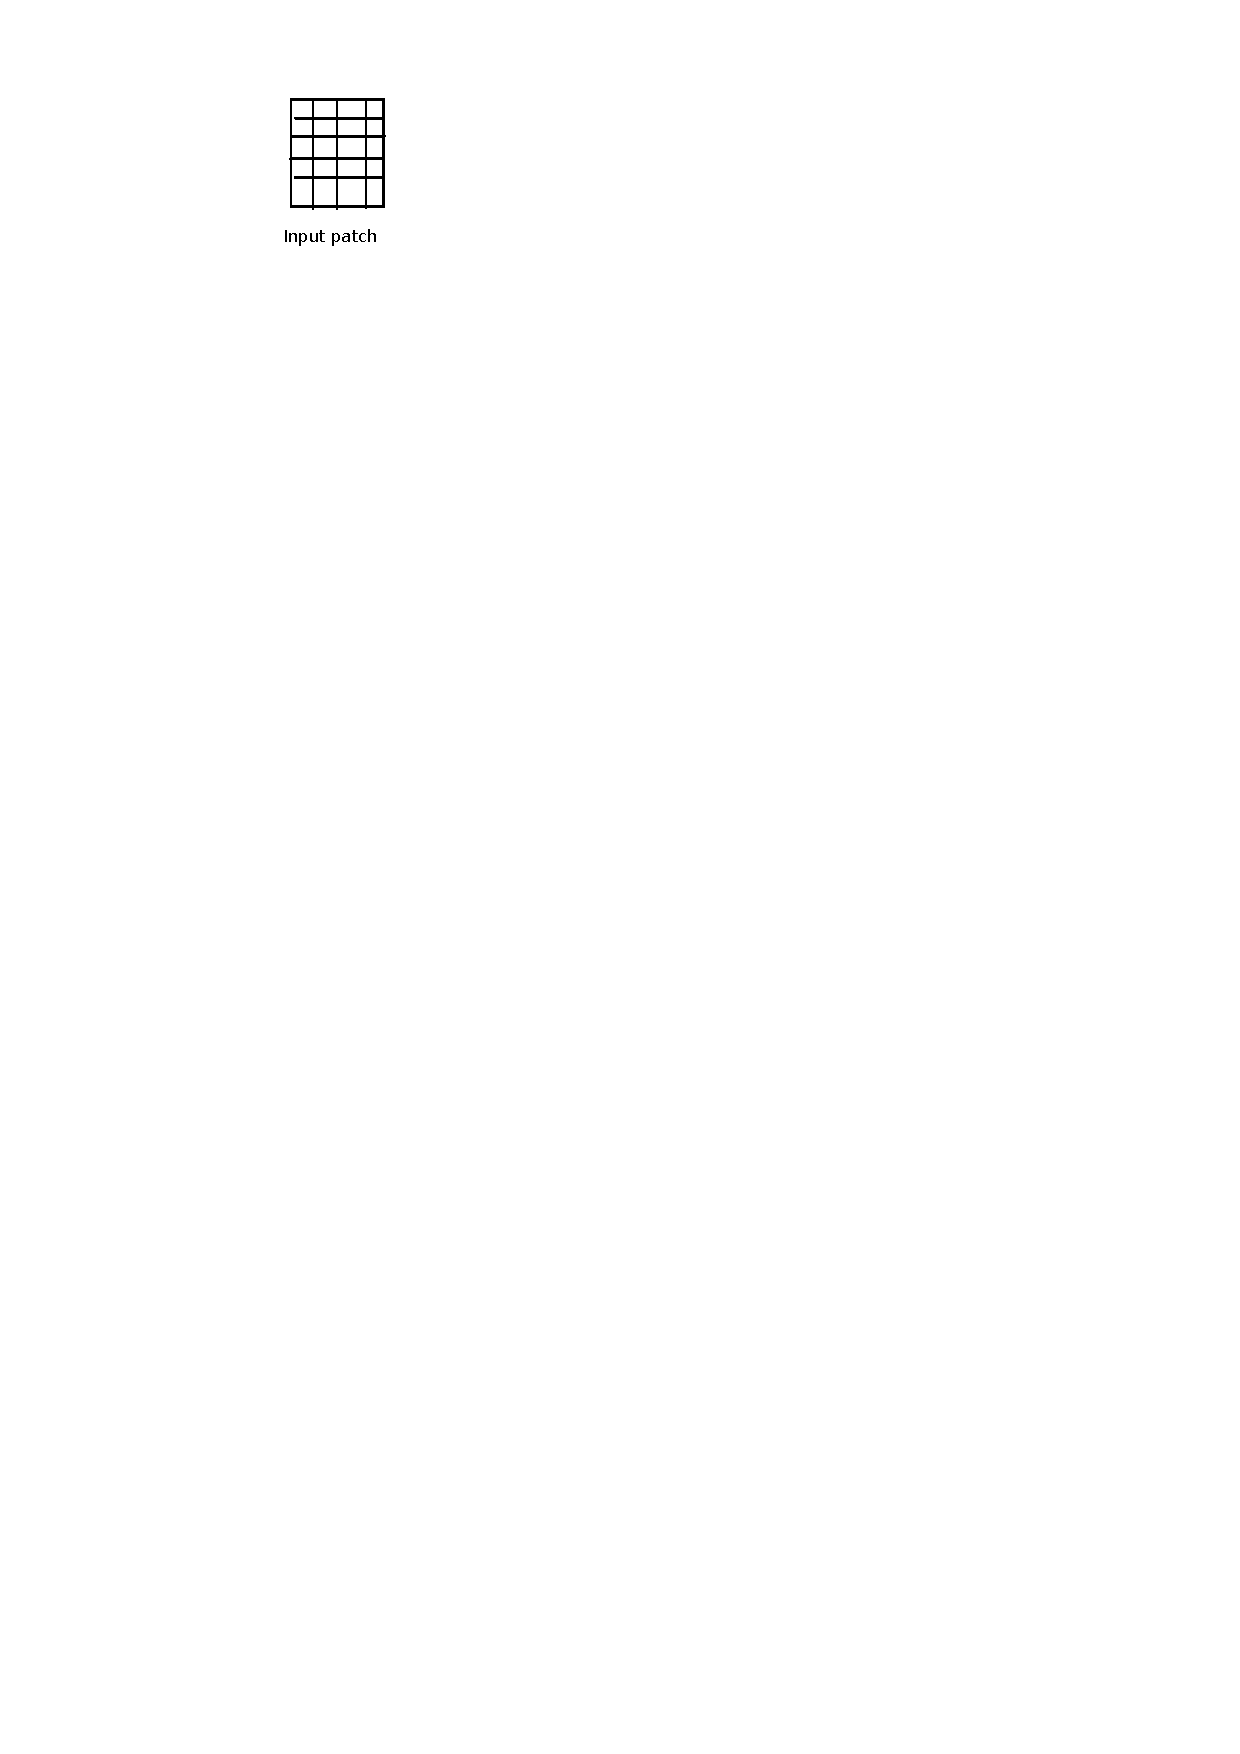
\includegraphics[trim={4.7cm, 25.5cm, 14.5cm, 2cm}, clip, width=1cm]{figure_slide}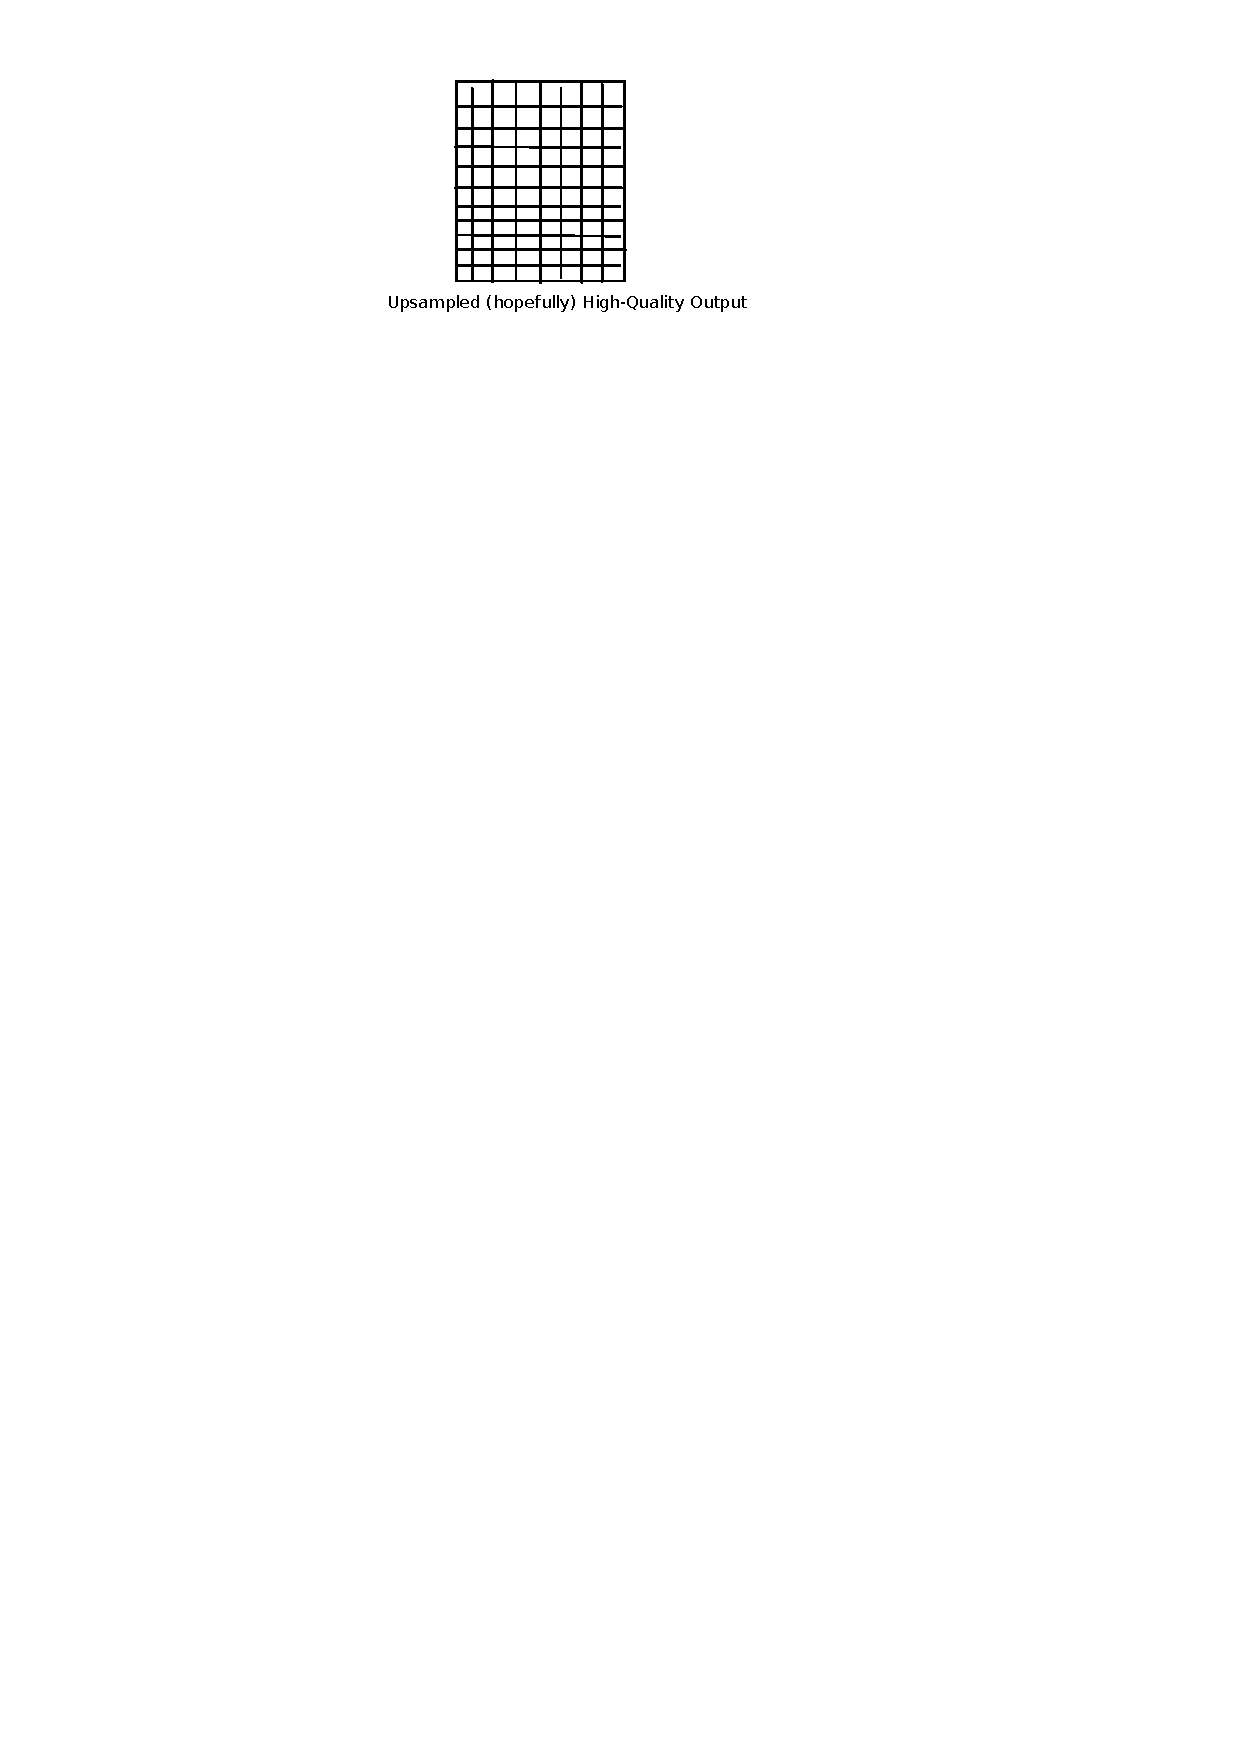
\includegraphics[trim={6.55cm, 24.3cm, 8.2cm, 1.2cm}, clip, width=3cm]{figure_output}
% 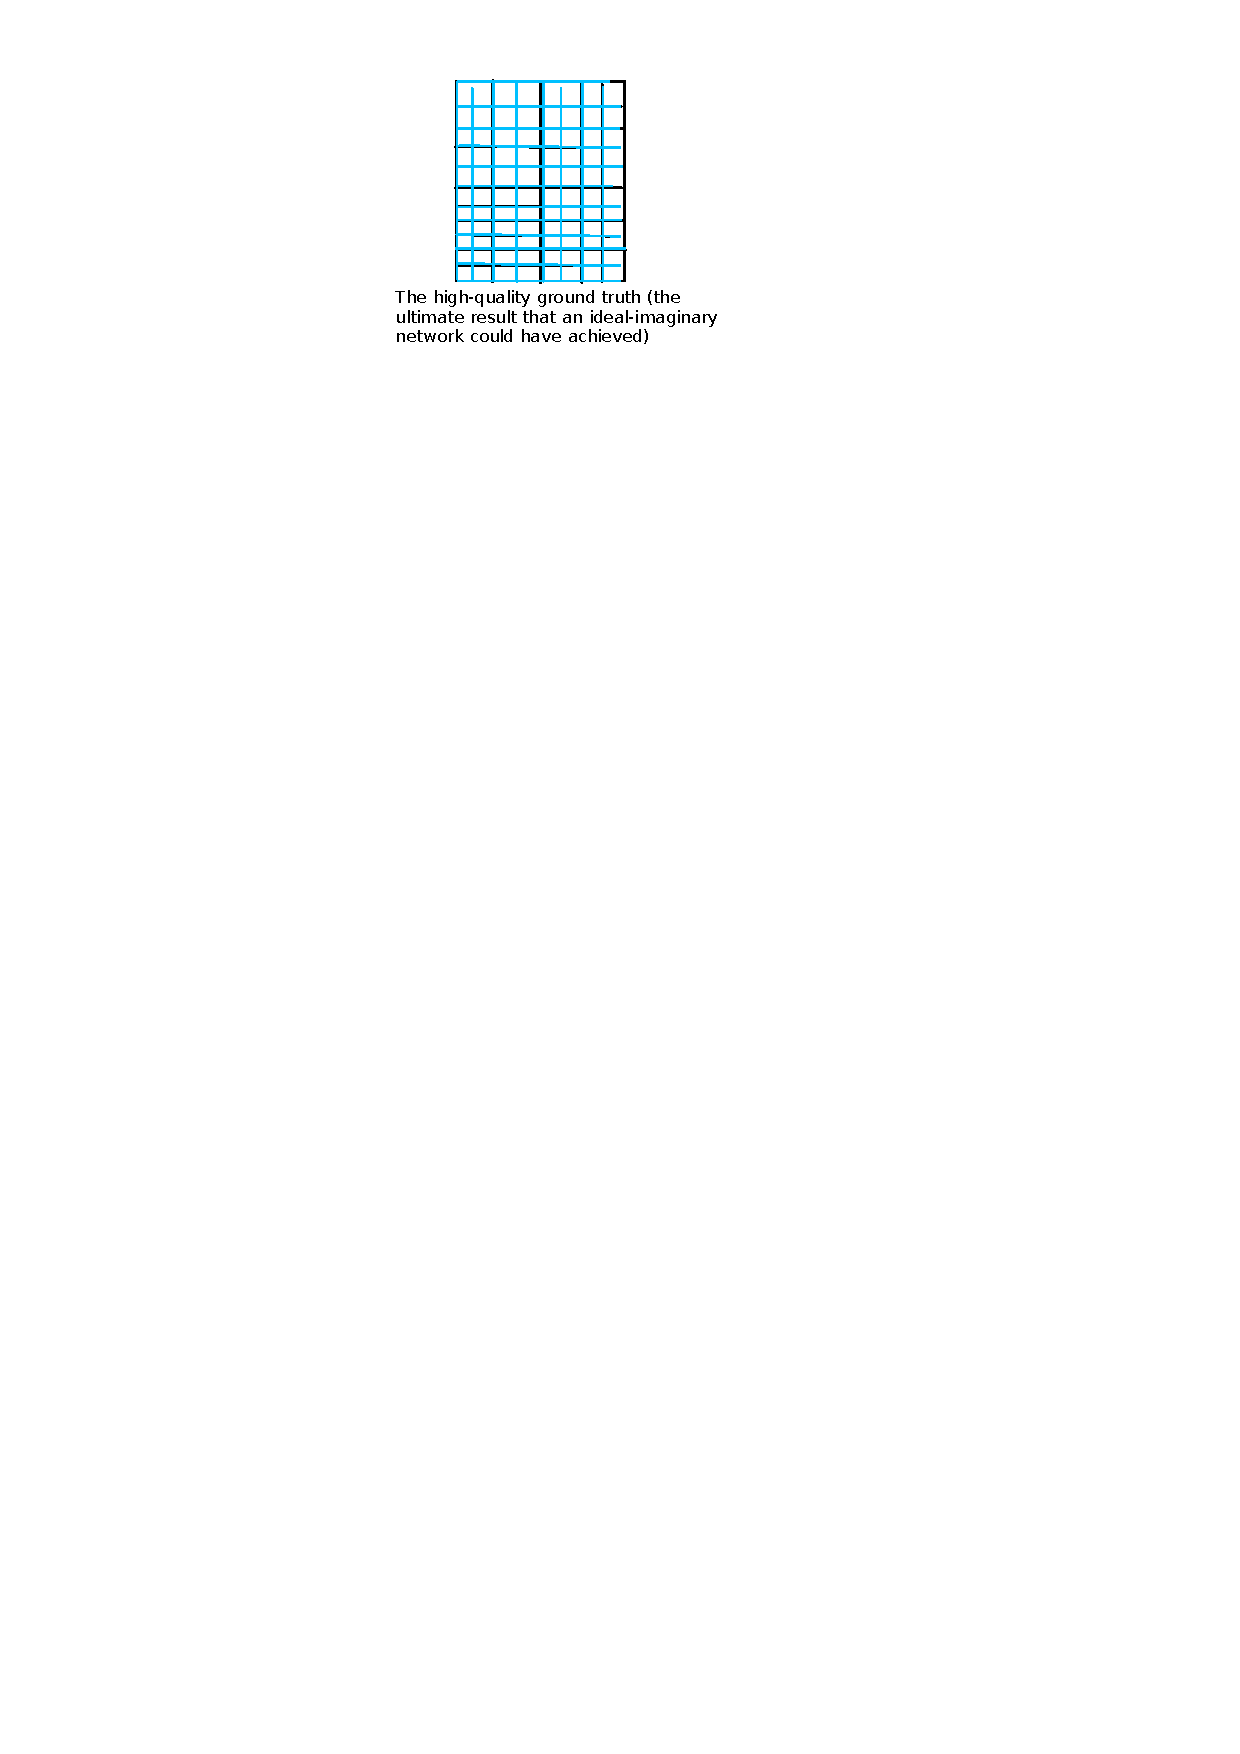
\includegraphics[trim={6.55cm, 23.3cm, 8.5cm, 1.2cm}, clip, width=3cm]{figure_gt}
% }
\visible<7->{
\item The Loss Function
	
	\only<8-14>{$X\rightarrow \text{Network's input}$}

		\only<9-14>{$\hat{Y}\rightarrow \text{Network's output}$}

		\only<10-14>{$Y\rightarrow \text{The correct answer}$}

		\only<11-14>{$W\rightarrow \text{Current network's weight}$}

		\only<12-14>{$Y=F(X, W)$}

		\only<13-14>{\small{The amount of update that must be applied to} $W~(i.e. \Delta W) = E(Y, \hat{Y})$; where $E\in[0,1]$}

		\only<14>{\small{The updated network's weights} $(i.e. W\prime) = W+\Delta W$}

		\onslide<15>{\textbf{How to define $E(Y, \hat{Y})$}?}
}
\end{itemize}
\end{frame}
%%%
\section{Previous Attempts}
\begin{frame}
	\frametitle{Ways to Define a Loss Function}
	\begin{itemize}
	\visible<2->{\item Visible Error}

		\visible<3->{
			$\displaystyle E(Y, \hat{Y})=\frac{1}{M\times N}\sum_{i=1}^M{\sum_{j=1}^N{(Y(i, j)-\hat{Y}(i, j))^2}}$
			}
		\visible<4->{\item Quality Metrics}
		
		\visible<5->{
			$E(Y, \hat{Y})=SSIM(Y, \hat{Y})$[1]
			}

		\visible<6->{
			\begin{center}
				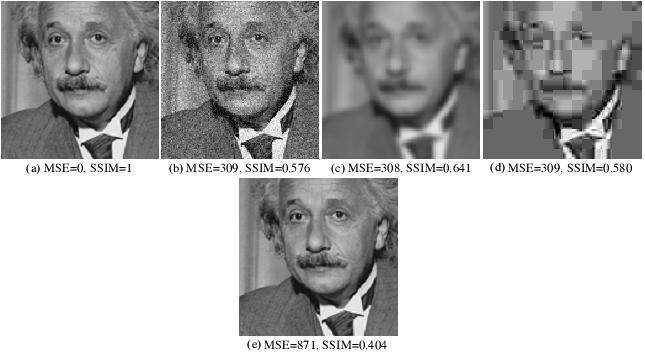
\includegraphics[width=8cm]{ssim_vs_mse}
			\end{center}
			}
	\end{itemize}
\end{frame}
%%%
\section{The Taken Approach}
\begin{frame}
\frametitle{Our Method}
\begin{itemize}
\visible<2->{
\item DCT
\begin{itemize}	
\visible<3->{
\item Expressive
\only<4-5>{

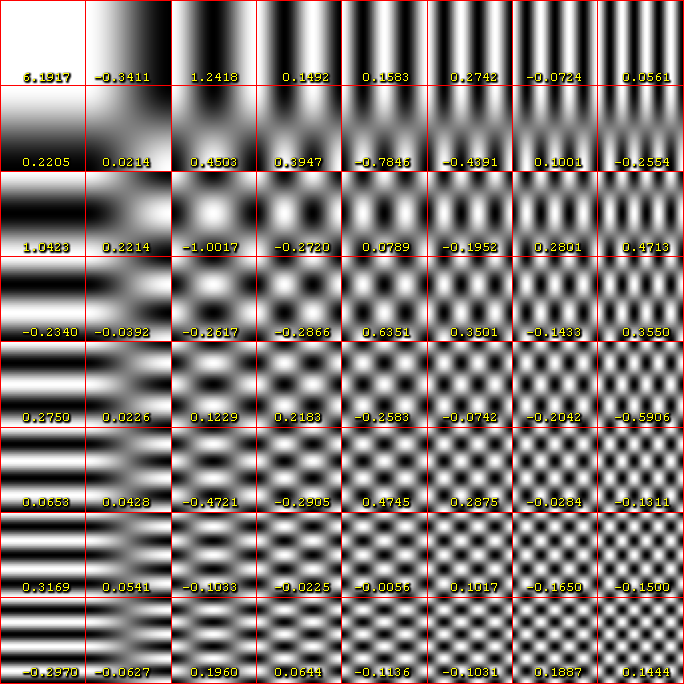
\includegraphics[width=3cm]{figure_dct_kernels}
}
\only<5>{
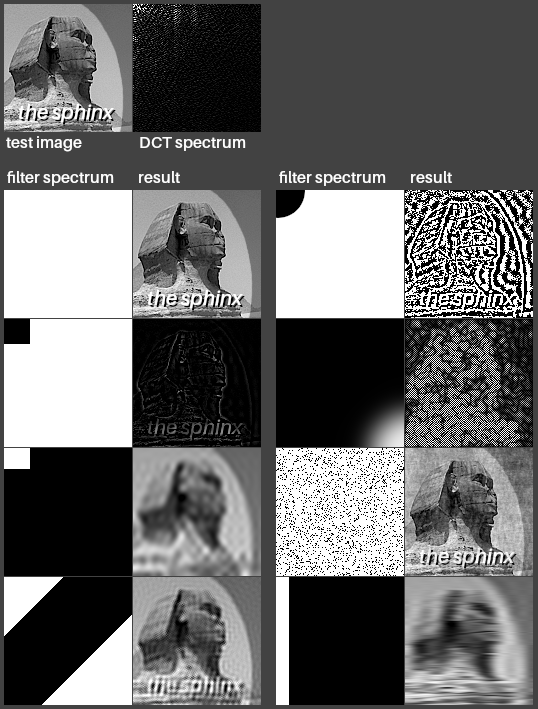
\includegraphics[width=5cm]{figure_dct_examples}
}
}
\visible<6->{
\item Fast!
}
\end{itemize}
}
\visible<7->{
\item Weighting the Important Components

	\visible<8->{
		Empirically determined compression quantization
		}

	\visible<9->{
		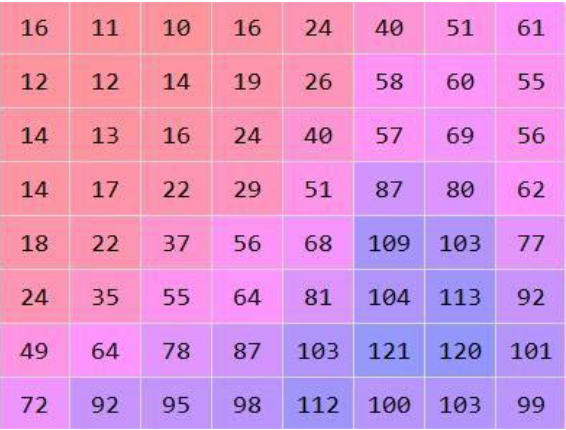
\includegraphics[width=3cm]{figure_JPEG_q}
		}
	
}
\end{itemize}

\end{frame}
%%%%
\begin{frame}
\frametitle{The Proposed Loss Function}
\only<1-4, 9>{
${Y, \hat{Y}}\rightarrow [0, 1]$
}
\vskip 0.5cm

	\only<2-4>{\textcolor[rgb]{0,0,1}{$\xrightarrow{(1)}$ compute $DCT(Y)$ and $DCT(\hat{Y})$}}
	
	\only<3-8>{\textcolor[rgb]{0,0.33,0.63}{$\xrightarrow{(2)}$ quantize $DCT(Y)$ and $DCT(\hat{Y})$}} 
	
	\only<4>{\textcolor[rgb]{0,0.63,0.33}{$\xrightarrow{(3)}$ compute the visible error between the quantized coefficients}}
	\vskip 0.5cm

	\only<6-8>{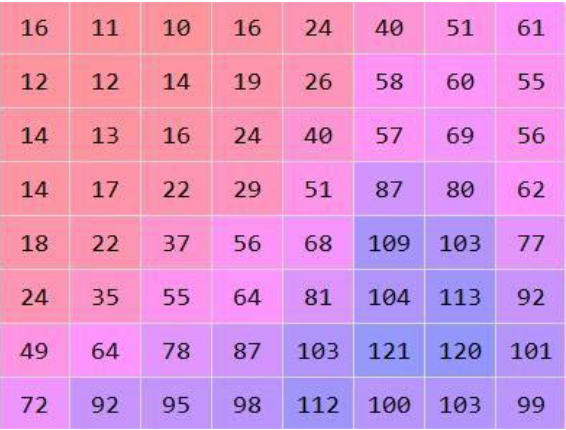
\includegraphics[width=2cm]{figure_JPEG_q}}\hskip 0.5cm \only<7-8>{$\xrightarrow{upsample}$ 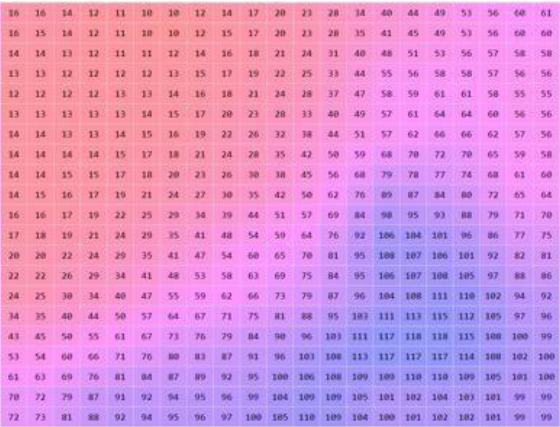
\includegraphics[width=4cm]{figure_JPEG_q_i}}

	\only<8>{$Q_l = \alpha \cdot \uparrow(Q)$}

	\only<9>{\fbox{\textcolor{blue}{\textbf{$\displaystyle popSR(Y, \hat{Y})=\frac{1}{21\times21}\sum_{i=1}^{21}\sum_{j=1}^{21}\left(\frac{DCT\left(Y\right)(i, j)}{Q_l(i, j)}-\frac{DCT\left(\hat{Y}\right)(i, j)}{Q_l(i, j)}\right)^2$}}}}
\end{frame}
%%%
\section{Results}
%%%%
\begin{frame}
\frametitle{Experimental Setup}
	\begin{itemize}
		\item train SRCNN [2] with MSE
		\item train SRCNN with popSR
		\item Timofte et. al [3] for train
		\item Set5 [4] Set14 [5] for test on various scales
	\end{itemize}
\end{frame}
\subsection{Qualitative}
\begin{frame}
	\frametitle{Sample Outputs}
	\only<1-3>{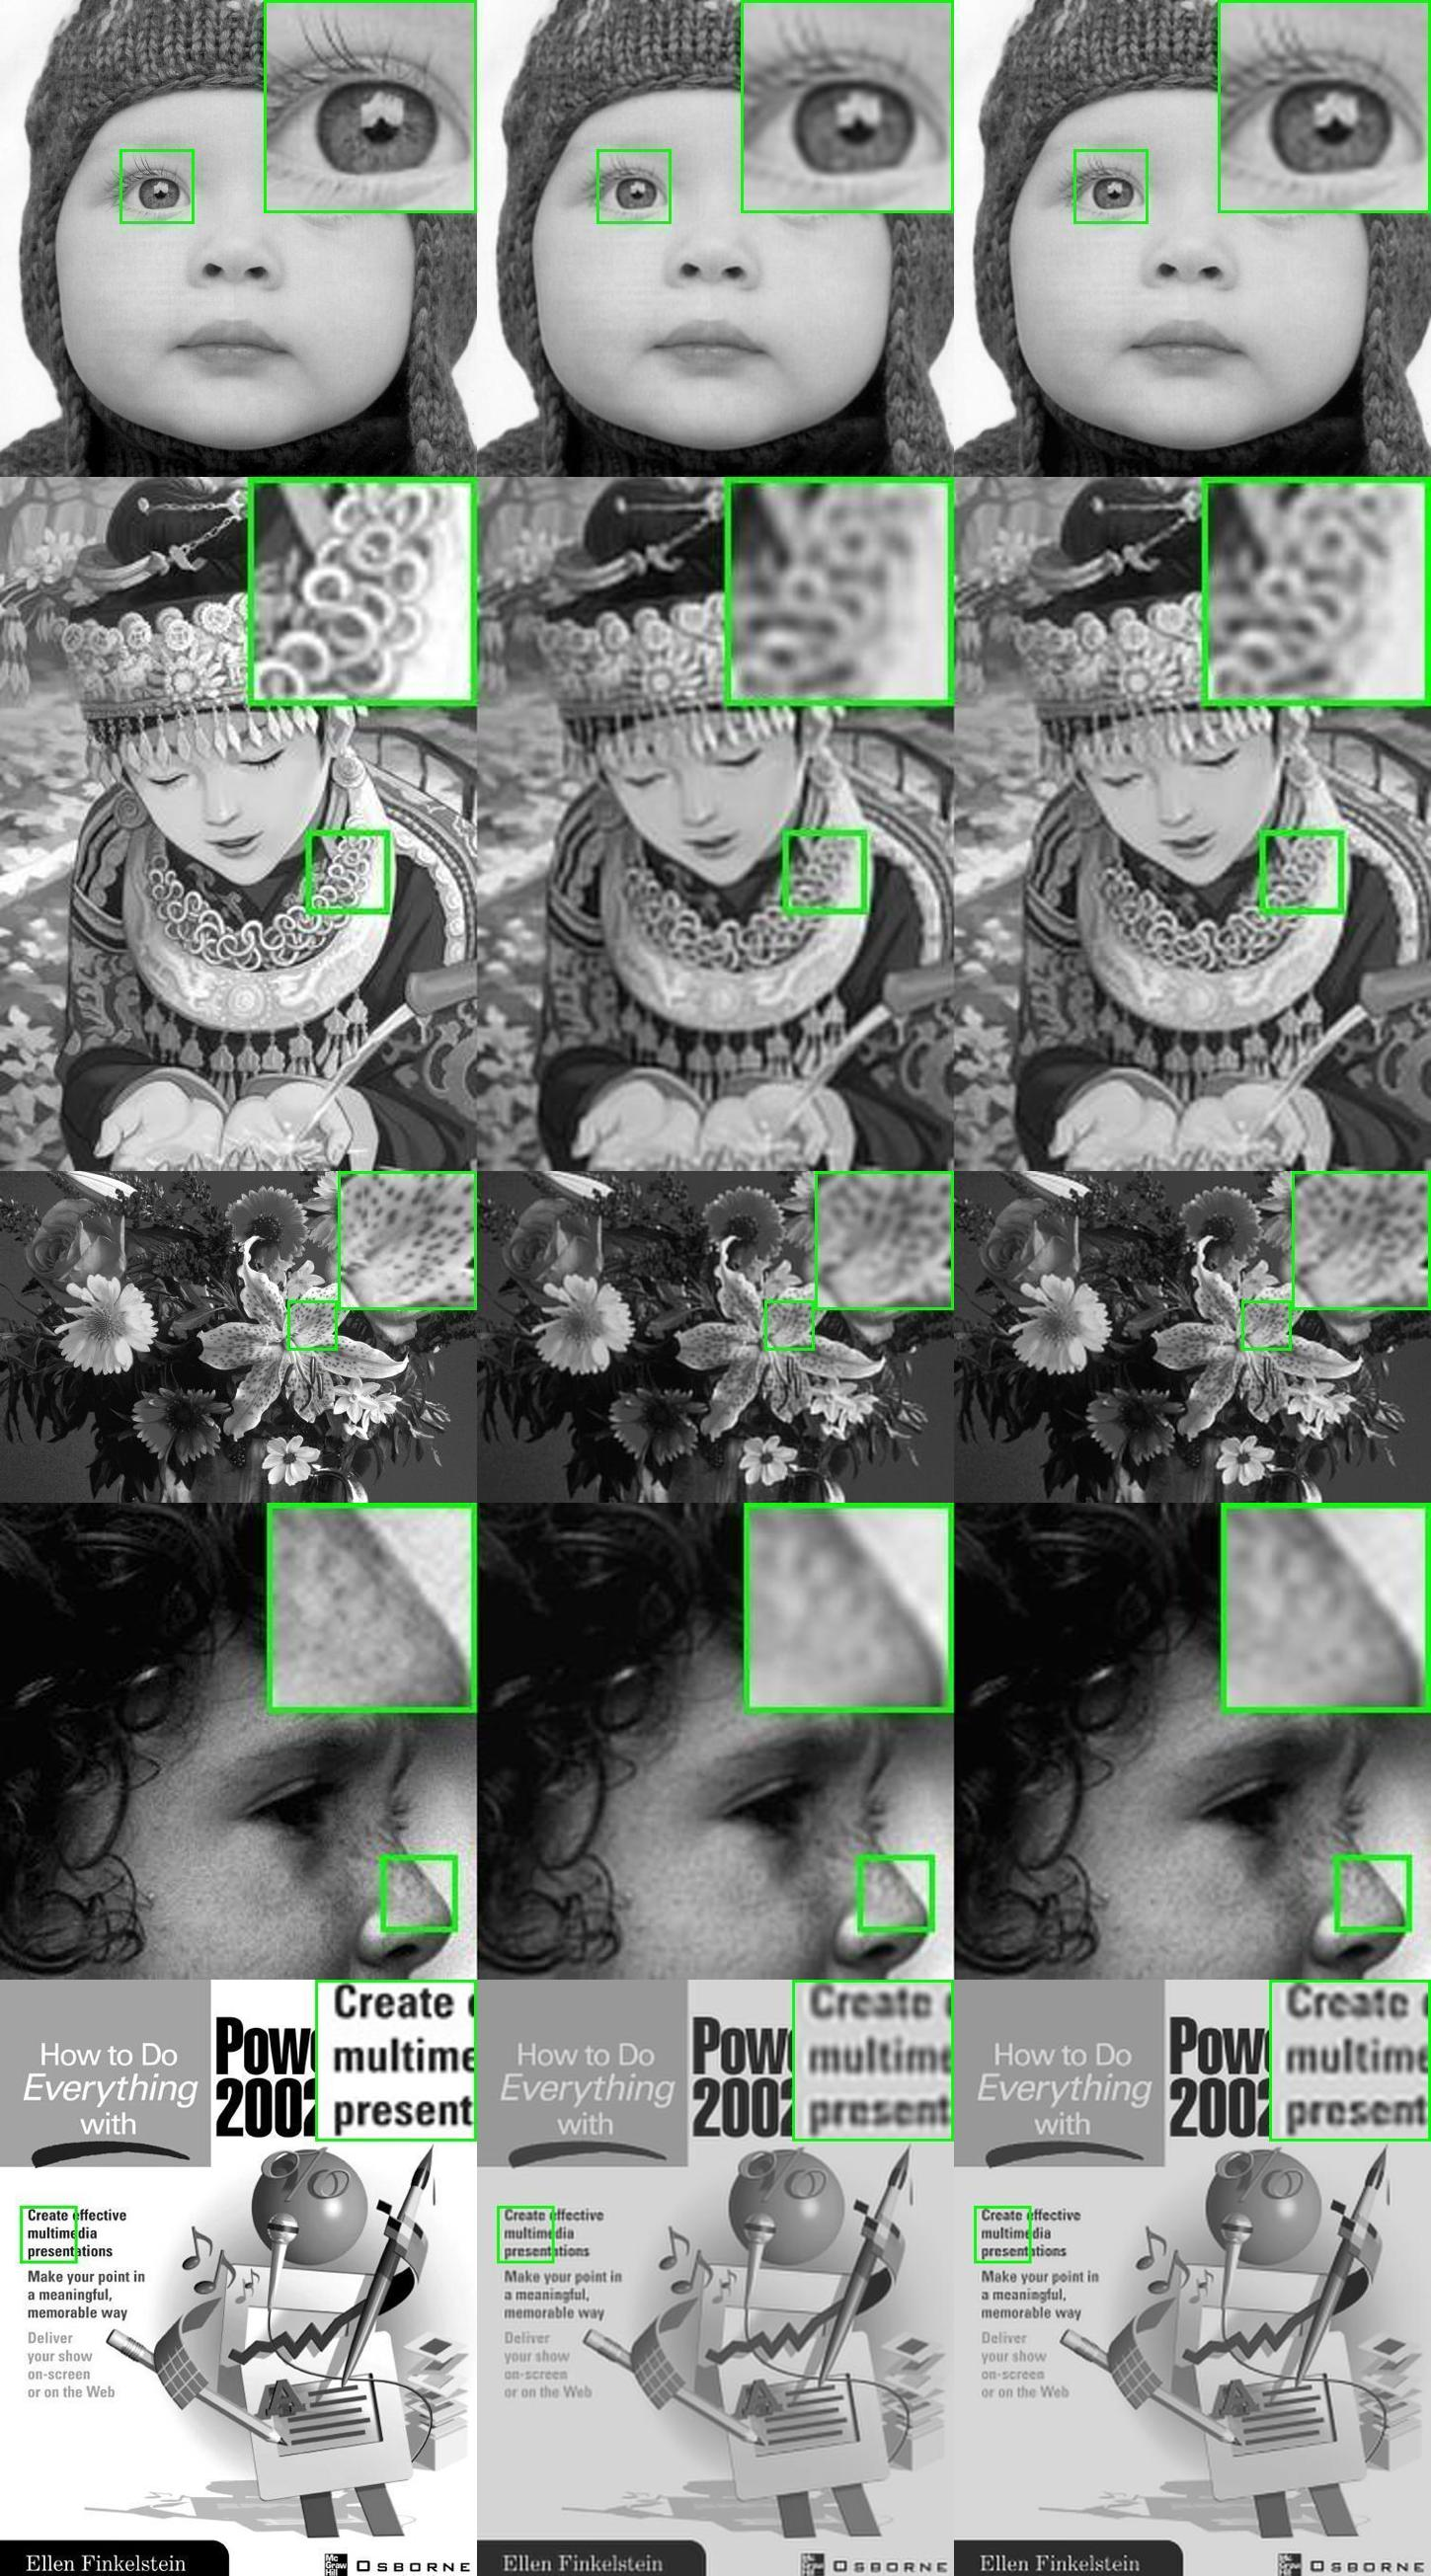
\includegraphics[height=6cm]{figure_sample}}
\only<2-3>{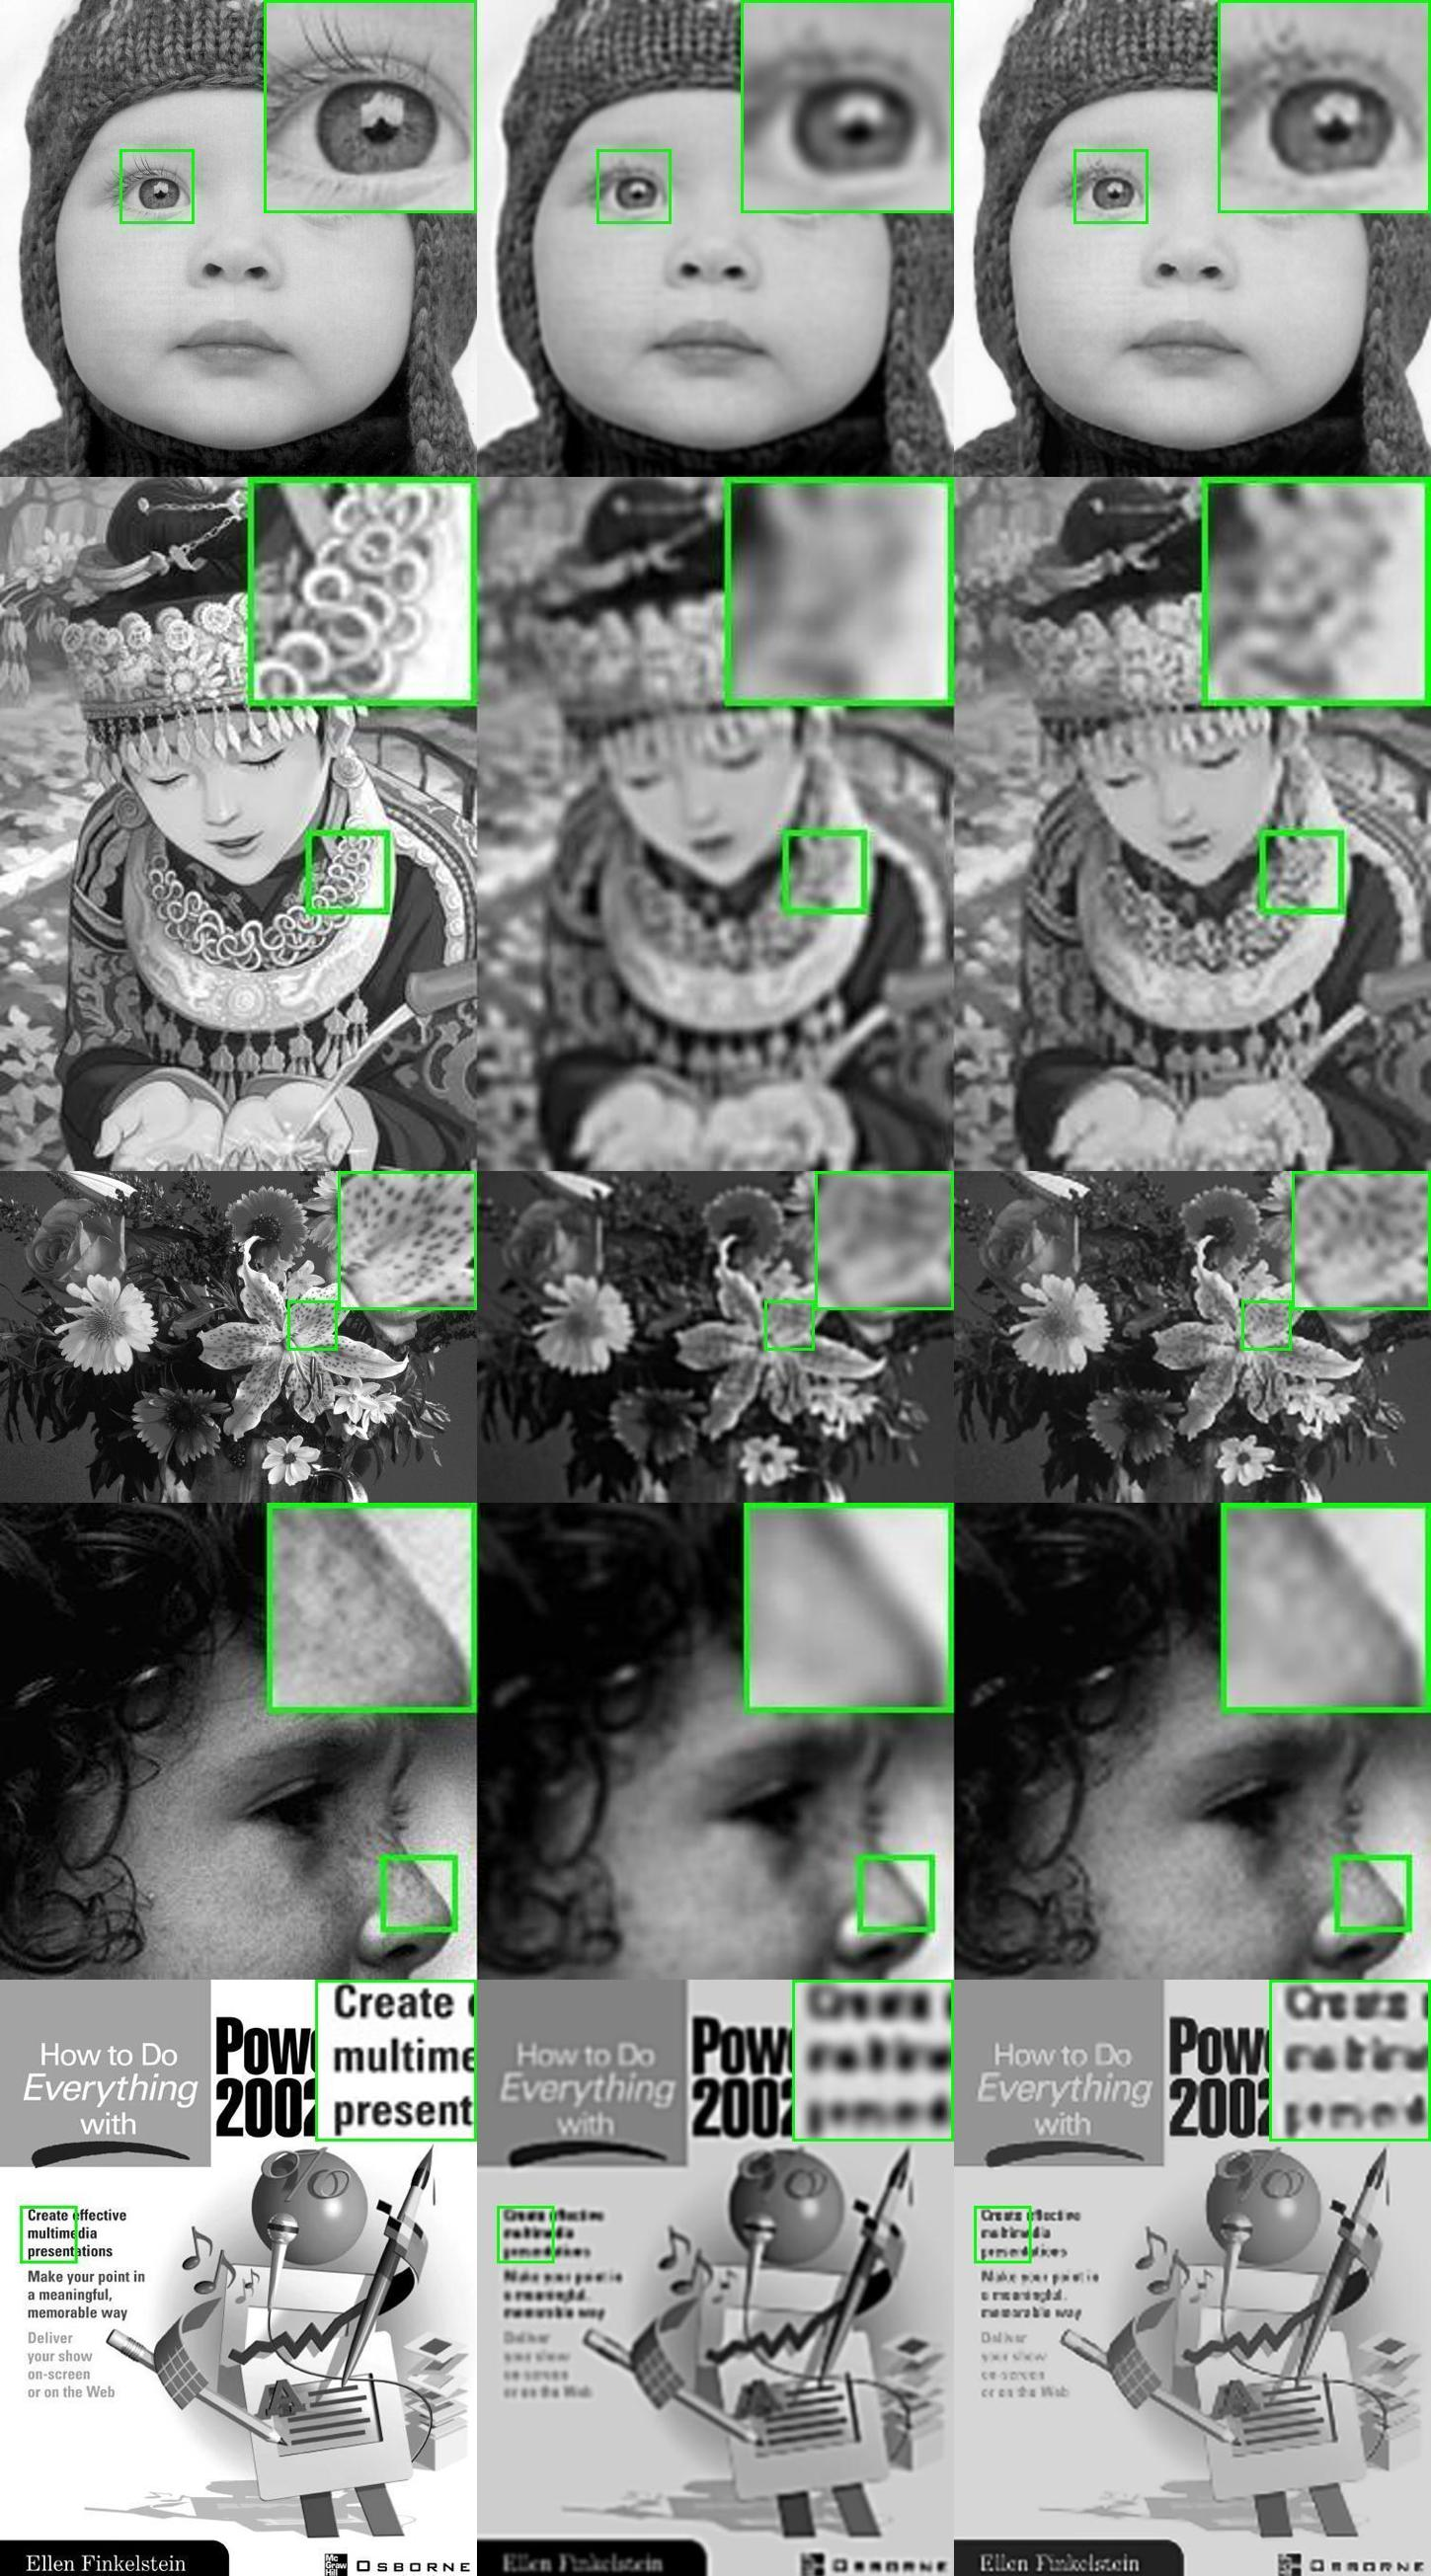
\includegraphics[height=6cm]{figure_sample_2}}
\only<3>{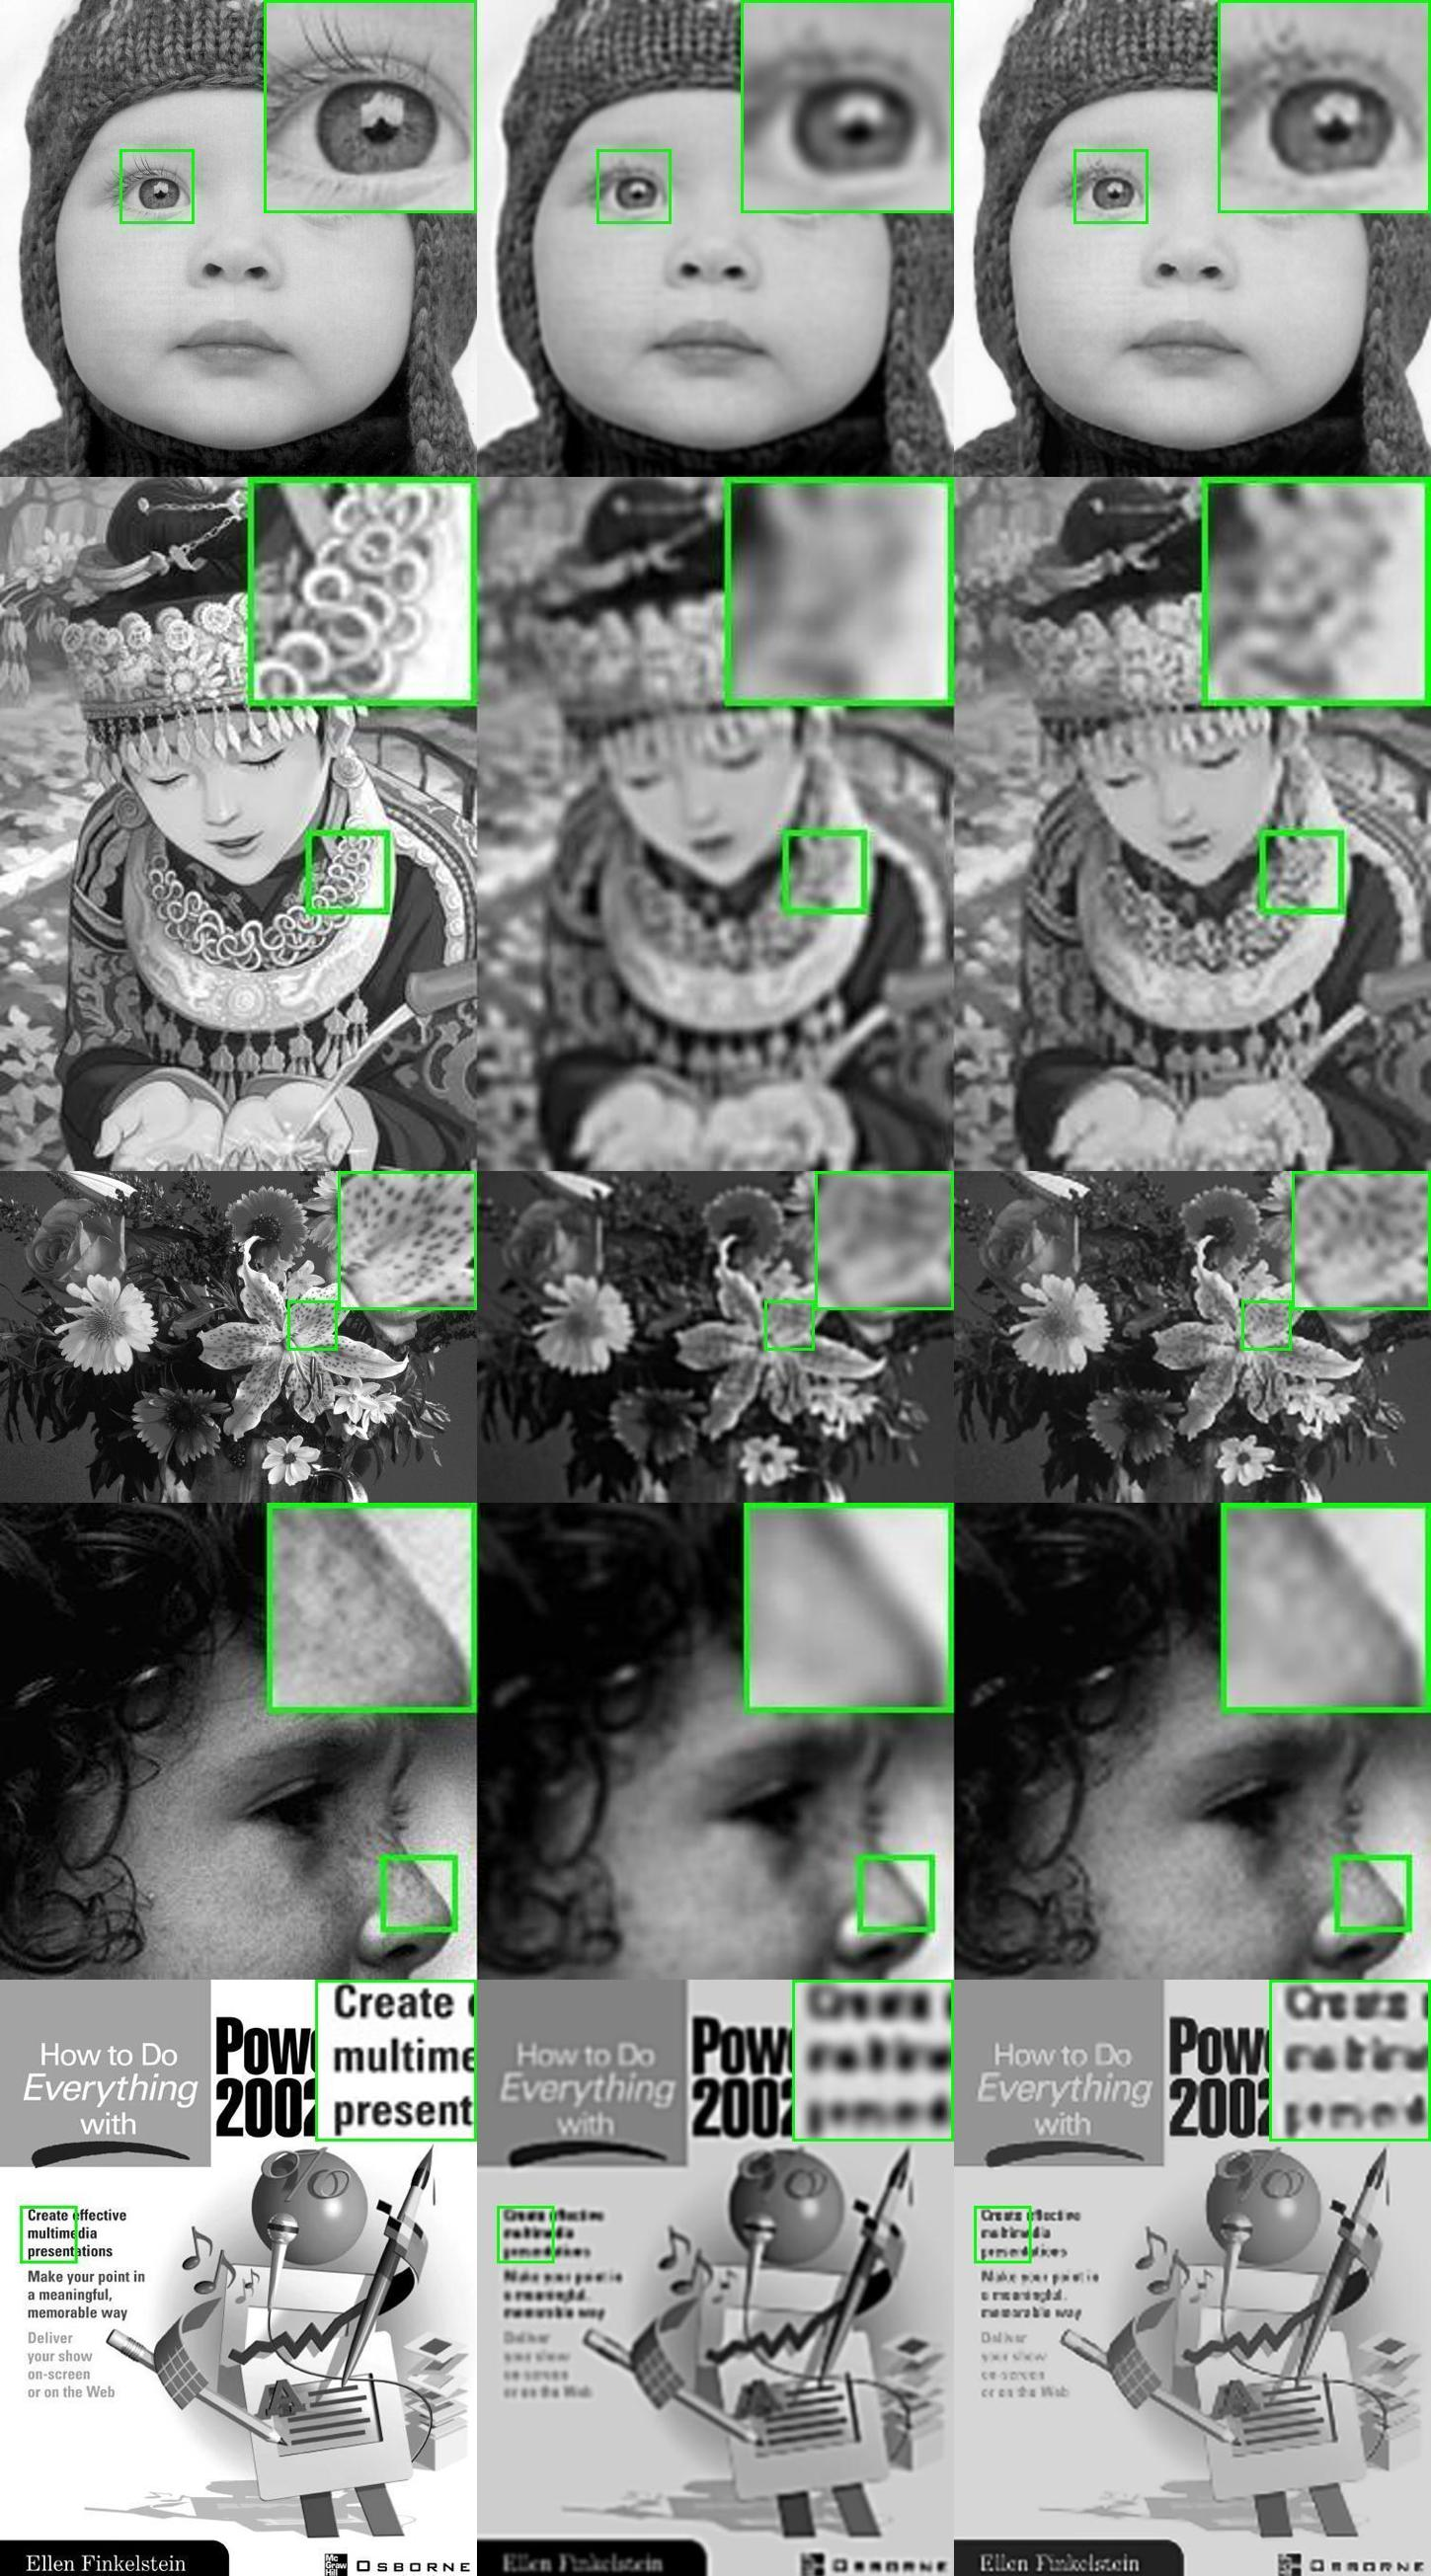
\includegraphics[height=6cm]{figure_sample_2}}
\end{frame}
%%%%
\subsection{Quantitative}
\begin{frame}
\frametitle{Objective Evaluation}
	\only<1>{
		\begin{itemize}
			\item Three metrics:
				\begin{itemize}
					\item PSNR
					\item SSIM
					\item GMSD [6]
				\end{itemize}
			\item Two datasets:
				\begin{itemize}
					\item set5
					\item set14
				\end{itemize}
			\item 3 scaling factors
				\begin{itemize}
					\item $2\uparrow$
					\item $3\uparrow$
					\item $4\uparrow$
				\end{itemize}
		\end{itemize}
		}
		\only<2>{set5 \& $2\uparrow$}
		
		\only<2>{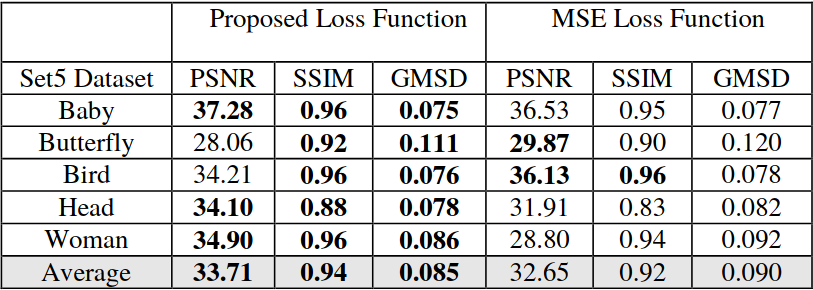
\includegraphics[width=5cm]{table_set5_2}}

		\only<3>{set5 \& $3\uparrow$}
		
		\only<3>{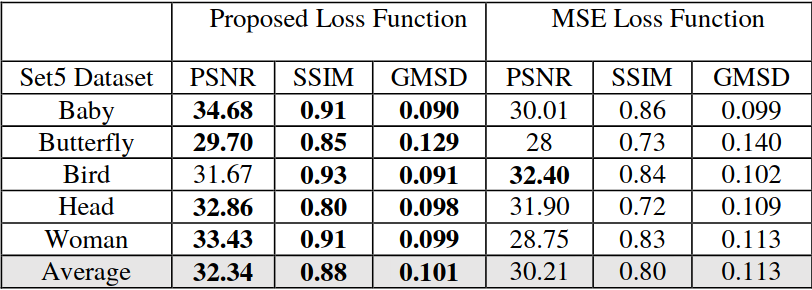
\includegraphics[width=5cm]{table_set5_3}}


		\only<4>{set5 \& $4\uparrow$}
		
		\only<4>{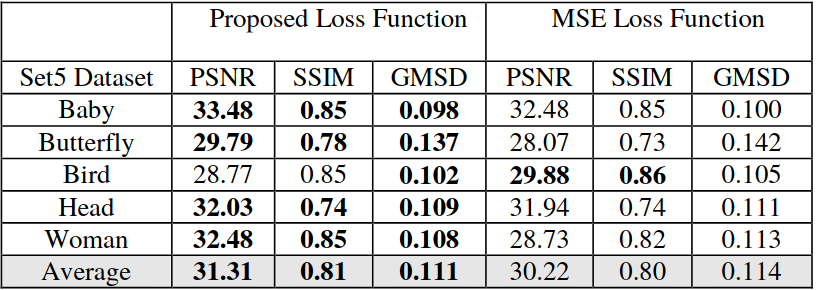
\includegraphics[width=5cm]{table_set5_4}}


		\only<5>{set14 \& $2\uparrow$}
		
		\only<5>{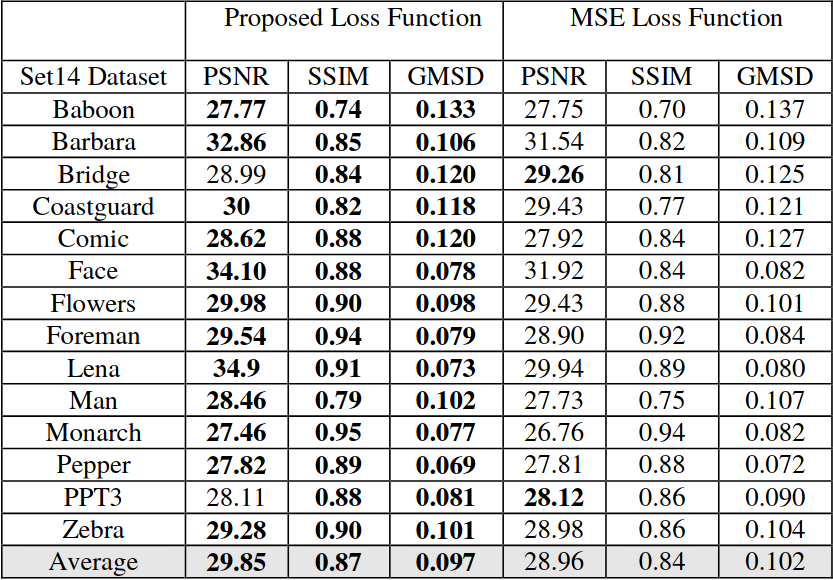
\includegraphics[width=5cm]{table_set14_2}}


		\only<6>{set14 \& $3\uparrow$}
		
		\only<6>{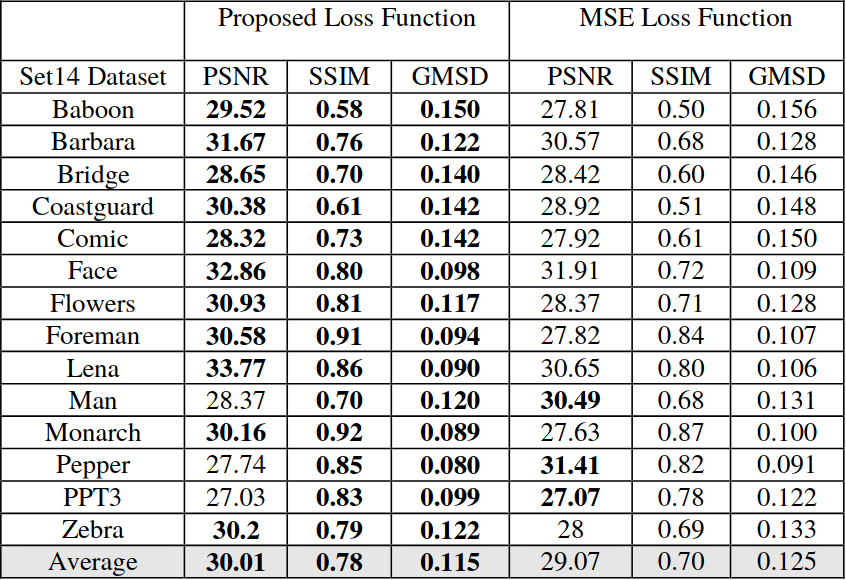
\includegraphics[width=5cm]{table_set14_3}}


		\only<7>{set14 \& $4\uparrow$}
		
		\only<7>{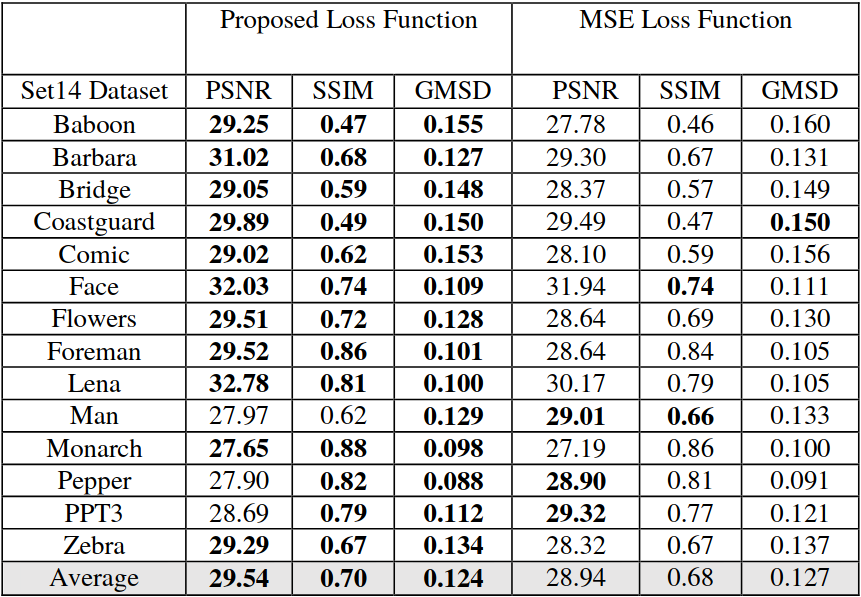
\includegraphics[width=5cm]{table_set14_4}}



			
\end{frame}
%%%%
\section{Conclusion\& Future Works}
%%%
\begin{frame}
	\frametitle{Conclusions}
	\begin{itemize}
		\item<1-> Perceptual
		\item<2-> Portable
		\item<3-> Efficient
		\item<4-> Faster Convergence
		\item<5-> Incorporating Color
			
	\end{itemize}
\end{frame}
\section*{References}
\begin{frame}
	\frametitle{Bibliography}
	\tiny{
	\begin{enumerate}
		\item Wang, Zhou, Alan C. Bovik, Hamid R. Sheikh, and Eero P. Simoncelli. "Image quality assessment: from error visibility to structural similarity." IEEE transactions on image processing 13, no. 4 (2004): 600-612.
                \item Dong, Chao, Chen Change Loy, Kaiming He, and Xiaoou Tang. "Learning a deep convolutional network for image super-resolution." In European conference on computer vision, pp. 184-199. Springer, Cham, 2014.
		\item Timofte, Radu, Vincent De Smet, and Luc Van Gool. "Anchored neighborhood regression for fast example-based super-resolution." In Proceedings of the IEEE international conference on computer vision, pp. 1920-1927. 2013.
		\item Bevilacqua, Marco, Aline Roumy, Christine Guillemot, and Marie Line Alberi-Morel. "Low-complexity single-image super-resolution based on nonnegative neighbor embedding." (2012): 135-1.
		\item Zeyde, Roman, Michael Elad, and Matan Protter. "On single image scale-up using sparse-representations." In International conference on curves and surfaces, pp. 711-730. Springer, Berlin, Heidelberg, 2010.
		\item Xue, Wufeng, Lei Zhang, Xuanqin Mou, and Alan C. Bovik. "Gradient magnitude similarity deviation: A highly efficient perceptual image quality index." IEEE Transactions on Image Processing 23, no. 2 (2013): 684-695.
	\end{enumerate}
	}
\end{frame}
\end{document}
